\chapter{Diseño y Arquitectura de la Solución}
\label{cap:03_diseno_arquitectura}

La solución contempla un frontend en React, un backend en Python y Flask, generación procedural, evaluación de mapas y un componente de aprendizaje automático.

\section{Arquitectura general del sistema (componentes y SBPMN)}

Rhyzome adopta una arquitectura cliente-servidor organizada mediante componentes modulares, los cuales permiten separar las responsabilidades de presentación, procesamiento, generación procedural, evaluación estructural y aprendizaje automático.

Esta organización facilita la integración de los diferentes componentes del sistema y permite mantener una separación entre la lógica de negocio y la interacción con el usuario.

\subsection{Arquitectura de componentes}
\label{subsec:arquitectura_componentes}

La Figura~\ref{fig:arquitectura_componentes} presenta la arquitectura de componentes correspondiente a la versión V2 del prototipo Rhyzome, identificando sus principales módulos y las relaciones existentes entre ellos.

\begin{landscape}
	\begin{figure}[H]
		\centering
		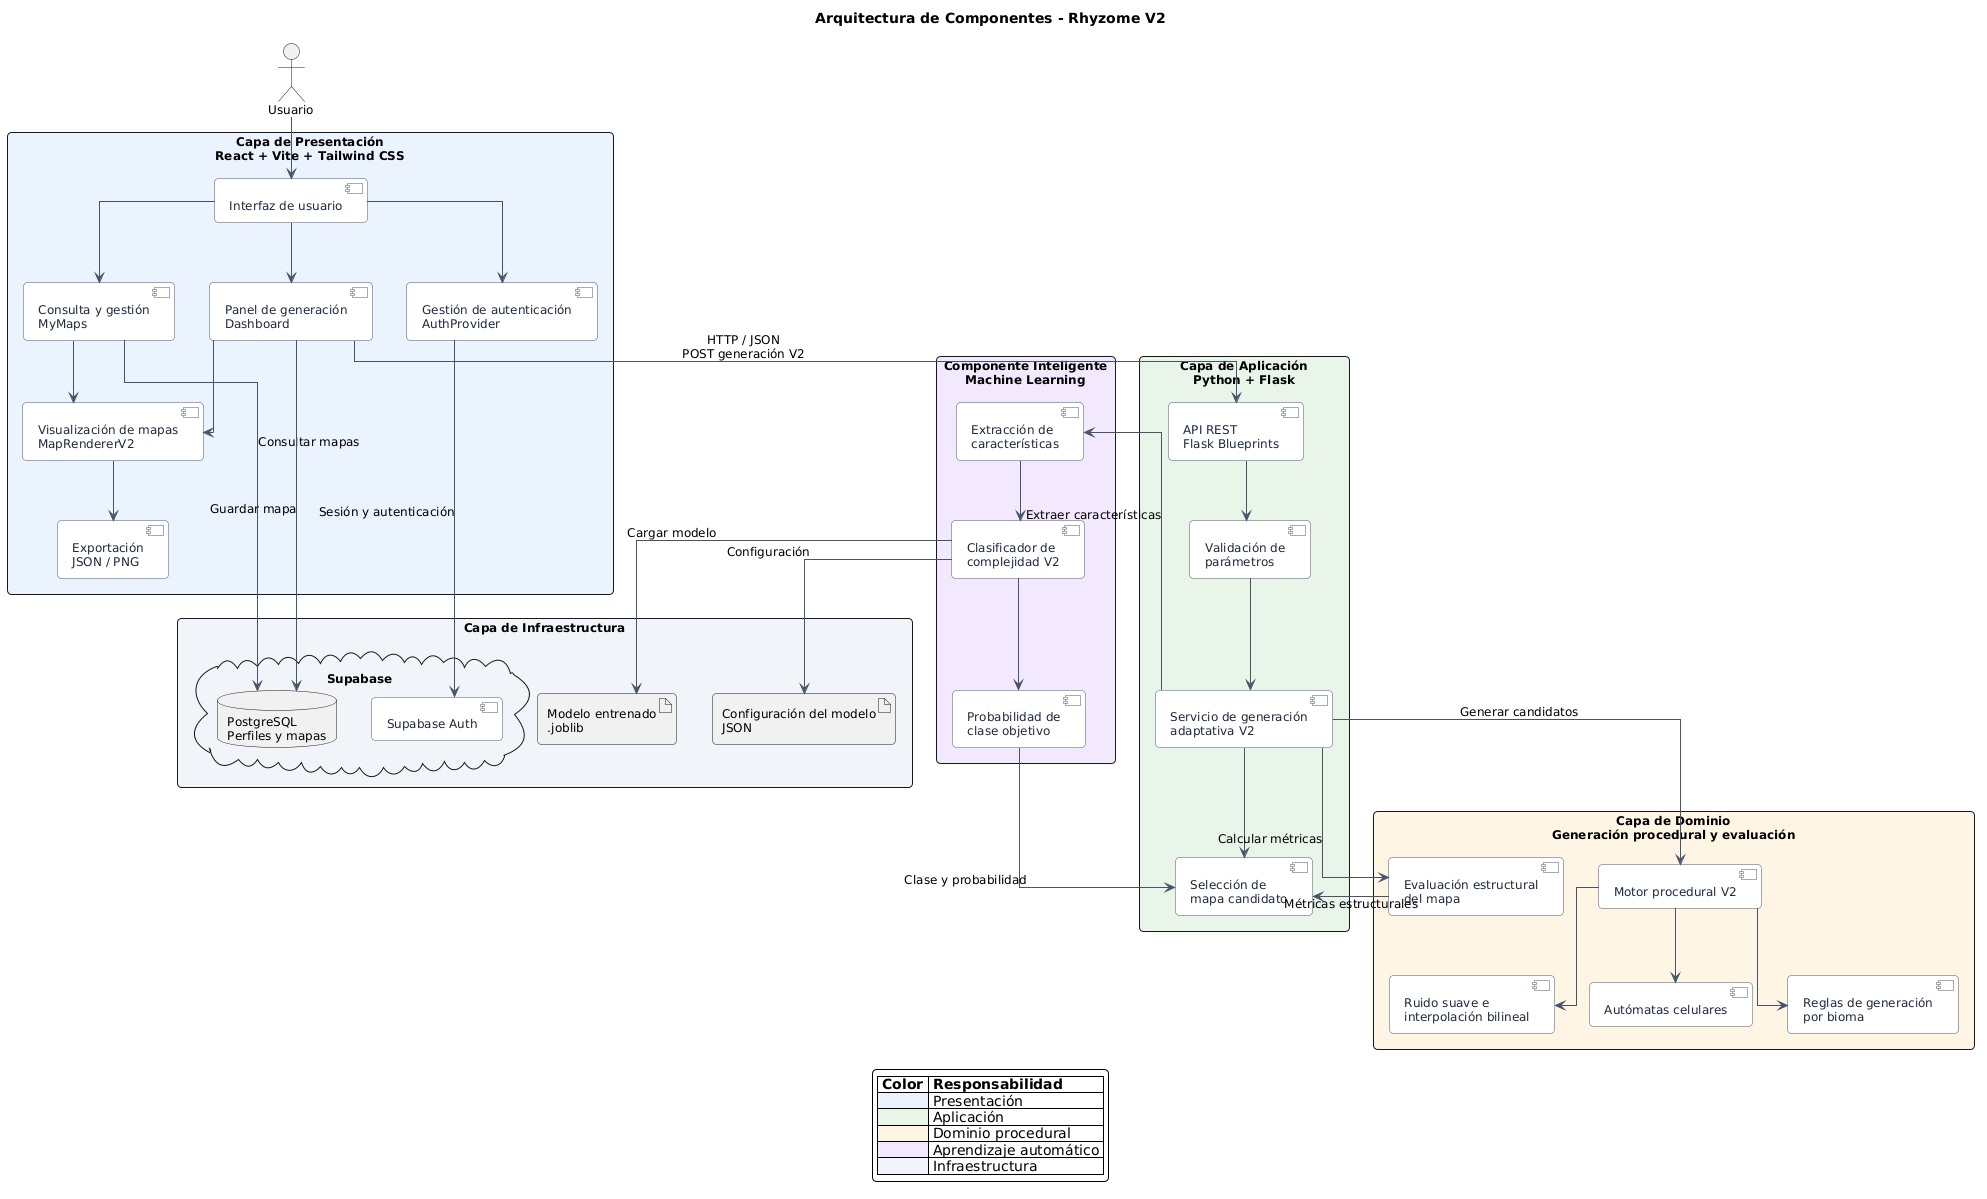
\includegraphics[width=\linewidth,height=0.78\vsize,keepaspectratio]{imagenes/ComponenteV2.png}
		\caption{Arquitectura de componentes de Rhyzome V2}
		\label{fig:arquitectura_componentes}
	\end{figure}
\end{landscape}

\FloatBarrier

La arquitectura se encuentra organizada en los siguientes bloques funcionales:

\begin{itemize}
	
	\item \textbf{Capa de presentación:}
	implementada mediante React, Vite y Tailwind CSS. Proporciona las funcionalidades de autenticación, configuración de parámetros, generación, visualización, consulta y exportación de mapas.
	
	\item \textbf{Capa de aplicación:}
	desarrollada mediante Python y Flask. Es responsable de exponer los servicios REST, validar los parámetros recibidos y coordinar el proceso de generación adaptativa.
	
	\item \textbf{Capa de dominio:}
	contiene los algoritmos de generación procedural, las reglas específicas de cada bioma y los mecanismos de evaluación estructural de los mapas. Su responsabilidad consiste en construir escenarios candidatos y determinar sus características.
	
	\item \textbf{Componente inteligente:}
	integra los mecanismos de extracción de características y clasificación mediante aprendizaje automático. El modelo estima la complejidad de los mapas candidatos y proporciona información para apoyar la selección del escenario final.
	
	\item \textbf{Capa de infraestructura:}
	proporciona los recursos necesarios para la autenticación, persistencia de información, almacenamiento de mapas y carga de los artefactos del modelo de aprendizaje automático.
	
\end{itemize}

La comunicación entre el frontend y el backend se realiza mediante servicios REST y estructuras de datos en formato JSON, permitiendo mantener independientes los componentes de presentación y procesamiento.

El modelo de aprendizaje automático clasifica los mapas candidatos; los algoritmos procedurales construyen los escenarios. El flujo de selección se desarrolla en la Sección~\ref{subsec:estrategia_generacion_adaptativa}.

\subsection{Flujo funcional del sistema (SBPMN)}
\label{subsec:flujo_funcional}

El flujo funcional de Rhyzome representa la secuencia de actividades que intervienen en la generación, evaluación y administración de mapas procedurales, identificando las responsabilidades del usuario, la interfaz web, los servicios de procesamiento y el componente inteligente.

La representación del proceso permite identificar los puntos de interacción, las decisiones asociadas a la generación procedural y los mecanismos de comunicación entre los componentes del sistema. La Figura~\ref{fig:flujo_funcional} presenta el flujo funcional correspondiente a la versión definitiva del prototipo Rhyzome.


\FloatBarrier
\clearpage

\begin{figure}[H]
	\centering
	
	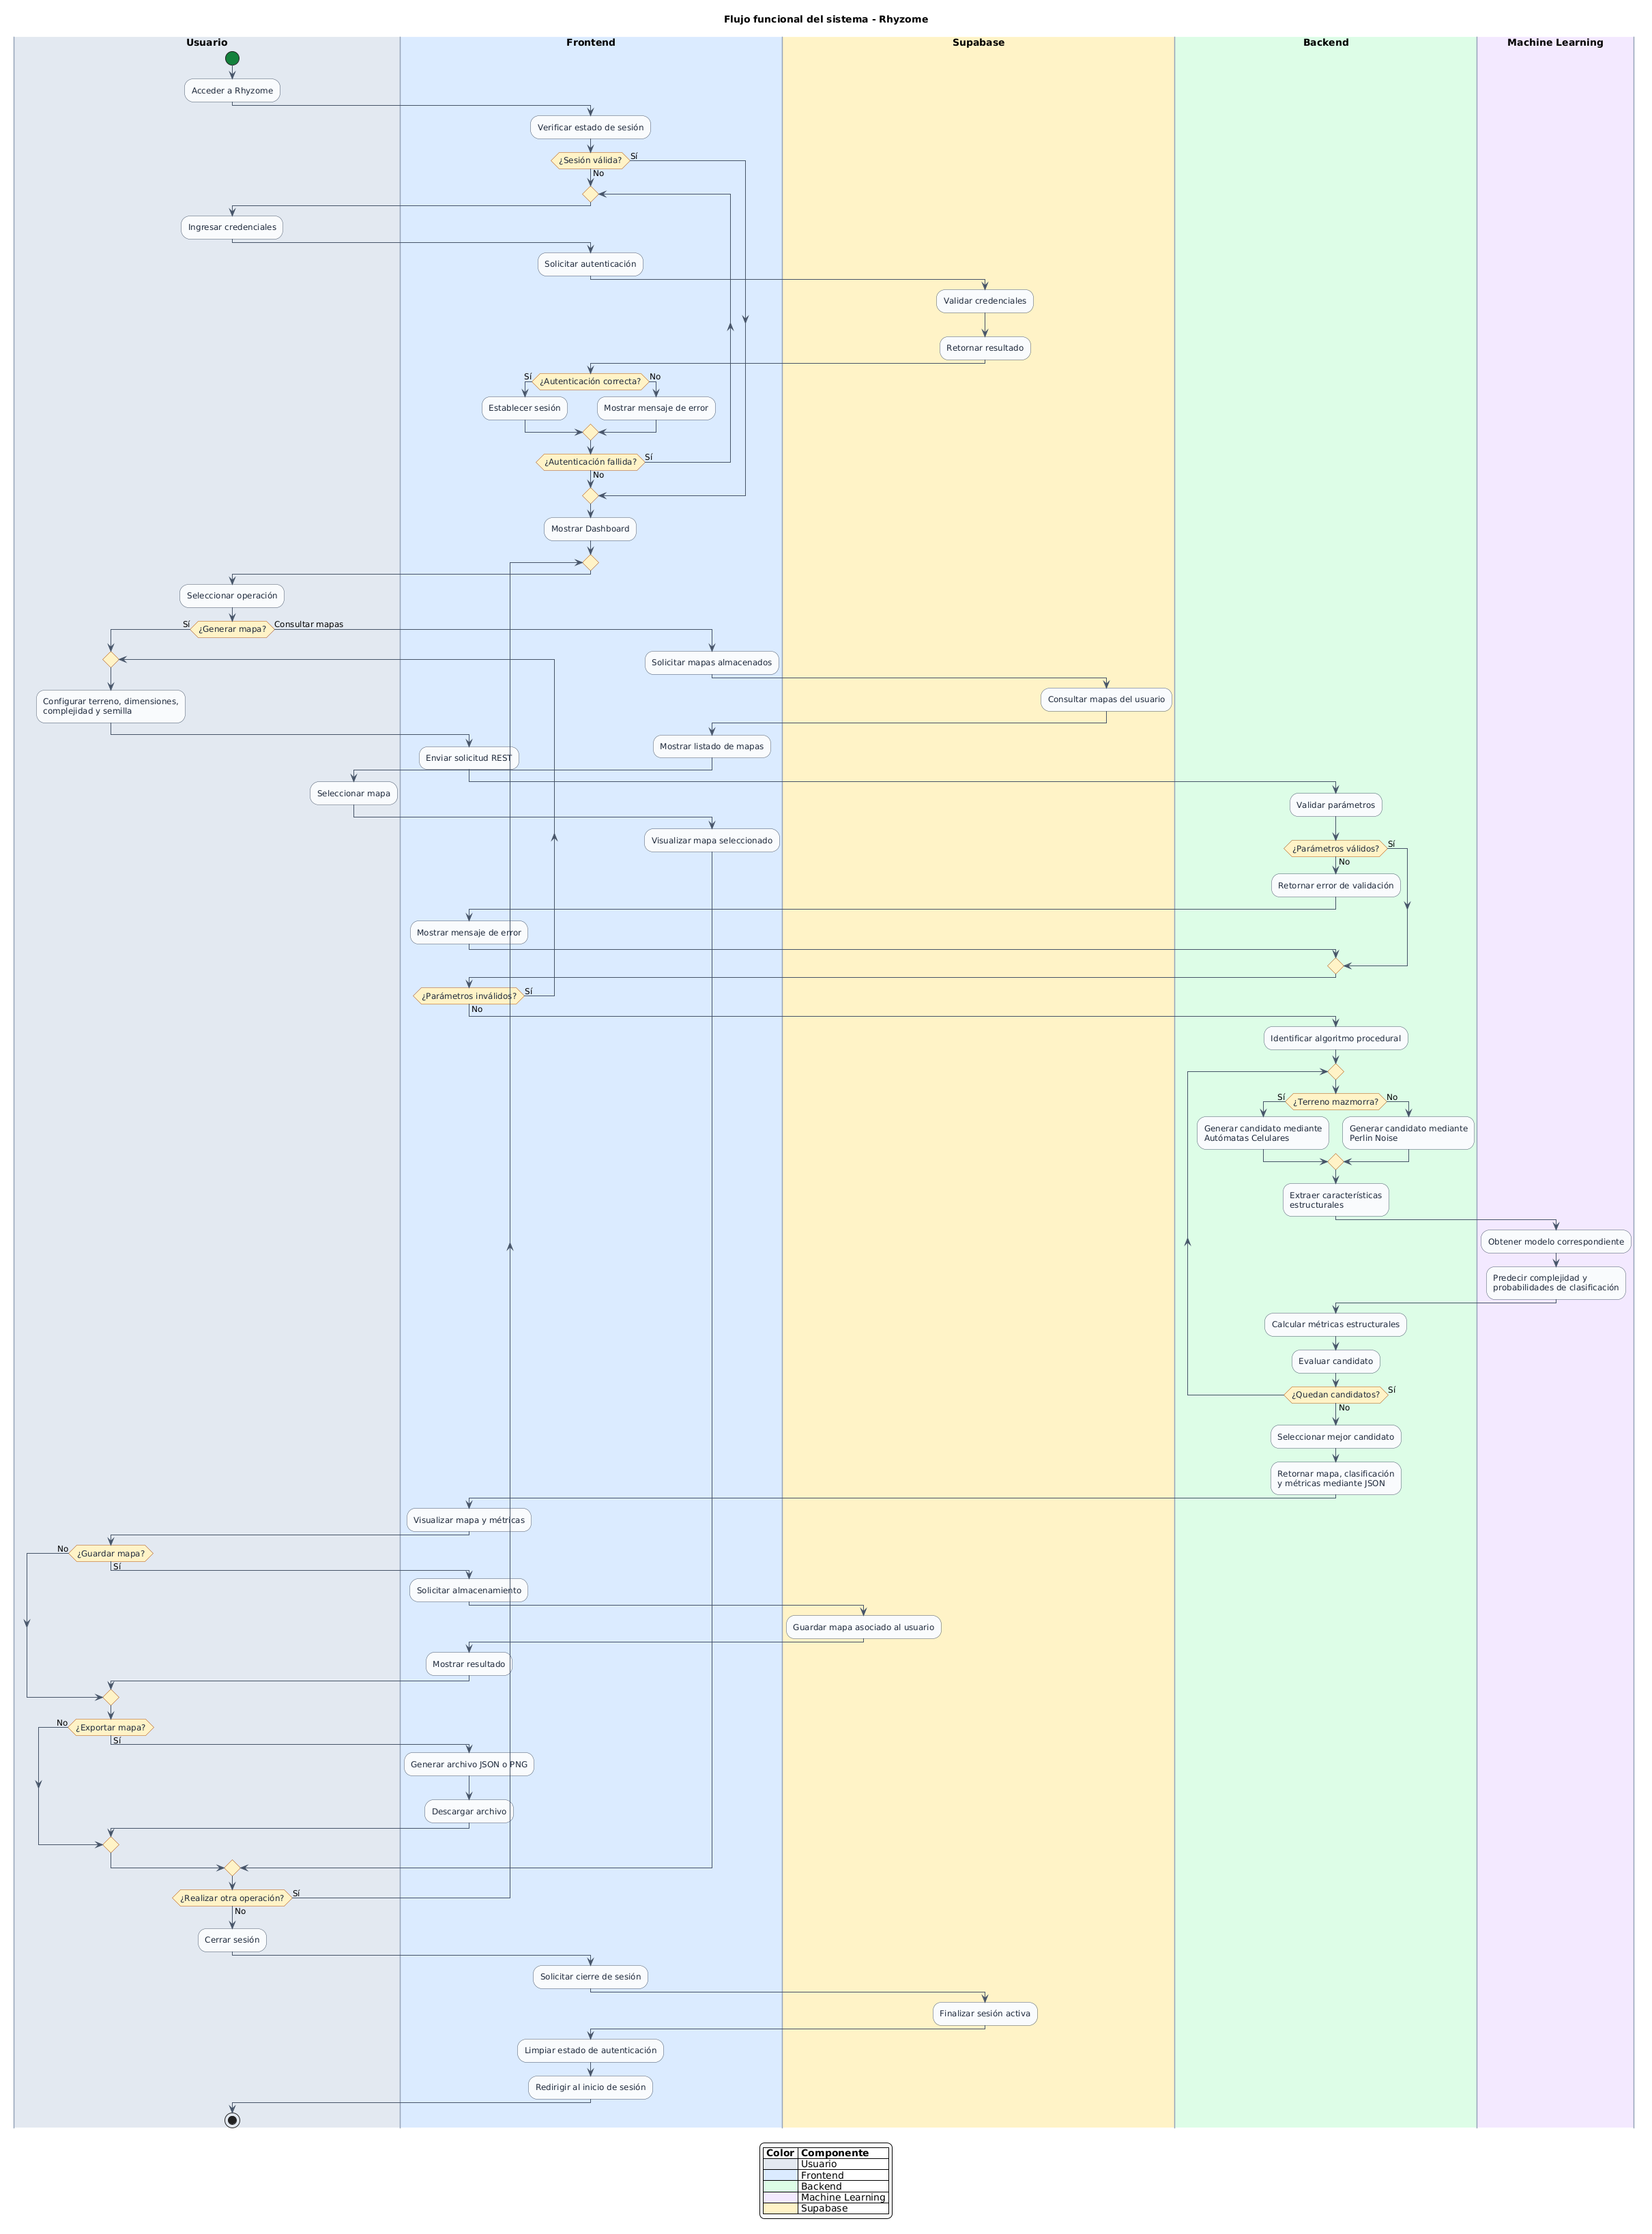
\includegraphics[
	width=\textwidth,
	height=0.90\textheight,
	keepaspectratio
	]{imagenes/flujo_funcional_rhyzome.png}
	
	\caption{Flujo funcional del sistema Rhyzome}
	\label{fig:flujo_funcional}
\end{figure}

\FloatBarrier
\clearpage


El proceso se organiza en cuatro etapas principales:

\begin{enumerate}
	
	\item \textbf{Acceso y configuración:}
	el usuario accede a la aplicación mediante una sesión válida y establece los parámetros necesarios para la generación del escenario.
	
	\item \textbf{Generación procedural:}
	el backend valida los parámetros recibidos y ejecuta el algoritmo correspondiente al tipo de terreno seleccionado, construyendo los mapas candidatos.
	
	\item \textbf{Evaluación y selección adaptativa:}
	se extraen las características estructurales de los candidatos y se utiliza el modelo de aprendizaje automático correspondiente para estimar su nivel de complejidad. Los resultados de clasificación y evaluación permiten seleccionar
	el escenario disponible que mejor se ajusta a los criterios establecidos.
	
	\item \textbf{Presentación y administración:}
	la interfaz visualiza el mapa seleccionado junto con sus métricas estructurales, proporcionando opciones de almacenamiento, consulta y exportación.
	
\end{enumerate}

El flujo contempla mecanismos de validación de parámetros y control de acceso, así como la separación entre las actividades de generación procedural y clasificación mediante aprendizaje automático.

Los detalles técnicos del mecanismo de generación adaptativa se desarrollan en la Sección~\ref{sec:integracion_ia}, mientras que la
evaluación experimental de los modelos y la validación funcional del sistema se presentan en los capítulos correspondientes.

\FloatBarrier

\section{Diagrama de despliegue}
\label{sec:diagrama_despliegue}

El despliegue de Rhyzome se fundamenta en una arquitectura distribuida que integra diferentes servicios en la nube para proporcionar las
funcionalidades de presentación, procesamiento, autenticación y persistencia de información.

Esta distribución permite mantener separados los componentes del frontend y backend, facilitando su administración, mantenimiento y actualización de manera independiente.

La Figura~\ref{fig:despliegue_rhyzome} presenta el diagrama de despliegue correspondiente a la versión V2 de Rhyzome, identificando los nodos de ejecución, los artefactos de software y los mecanismos de comunicación utilizados por el sistema.

\begin{landscape}
	\begin{figure}[H]
		\centering
		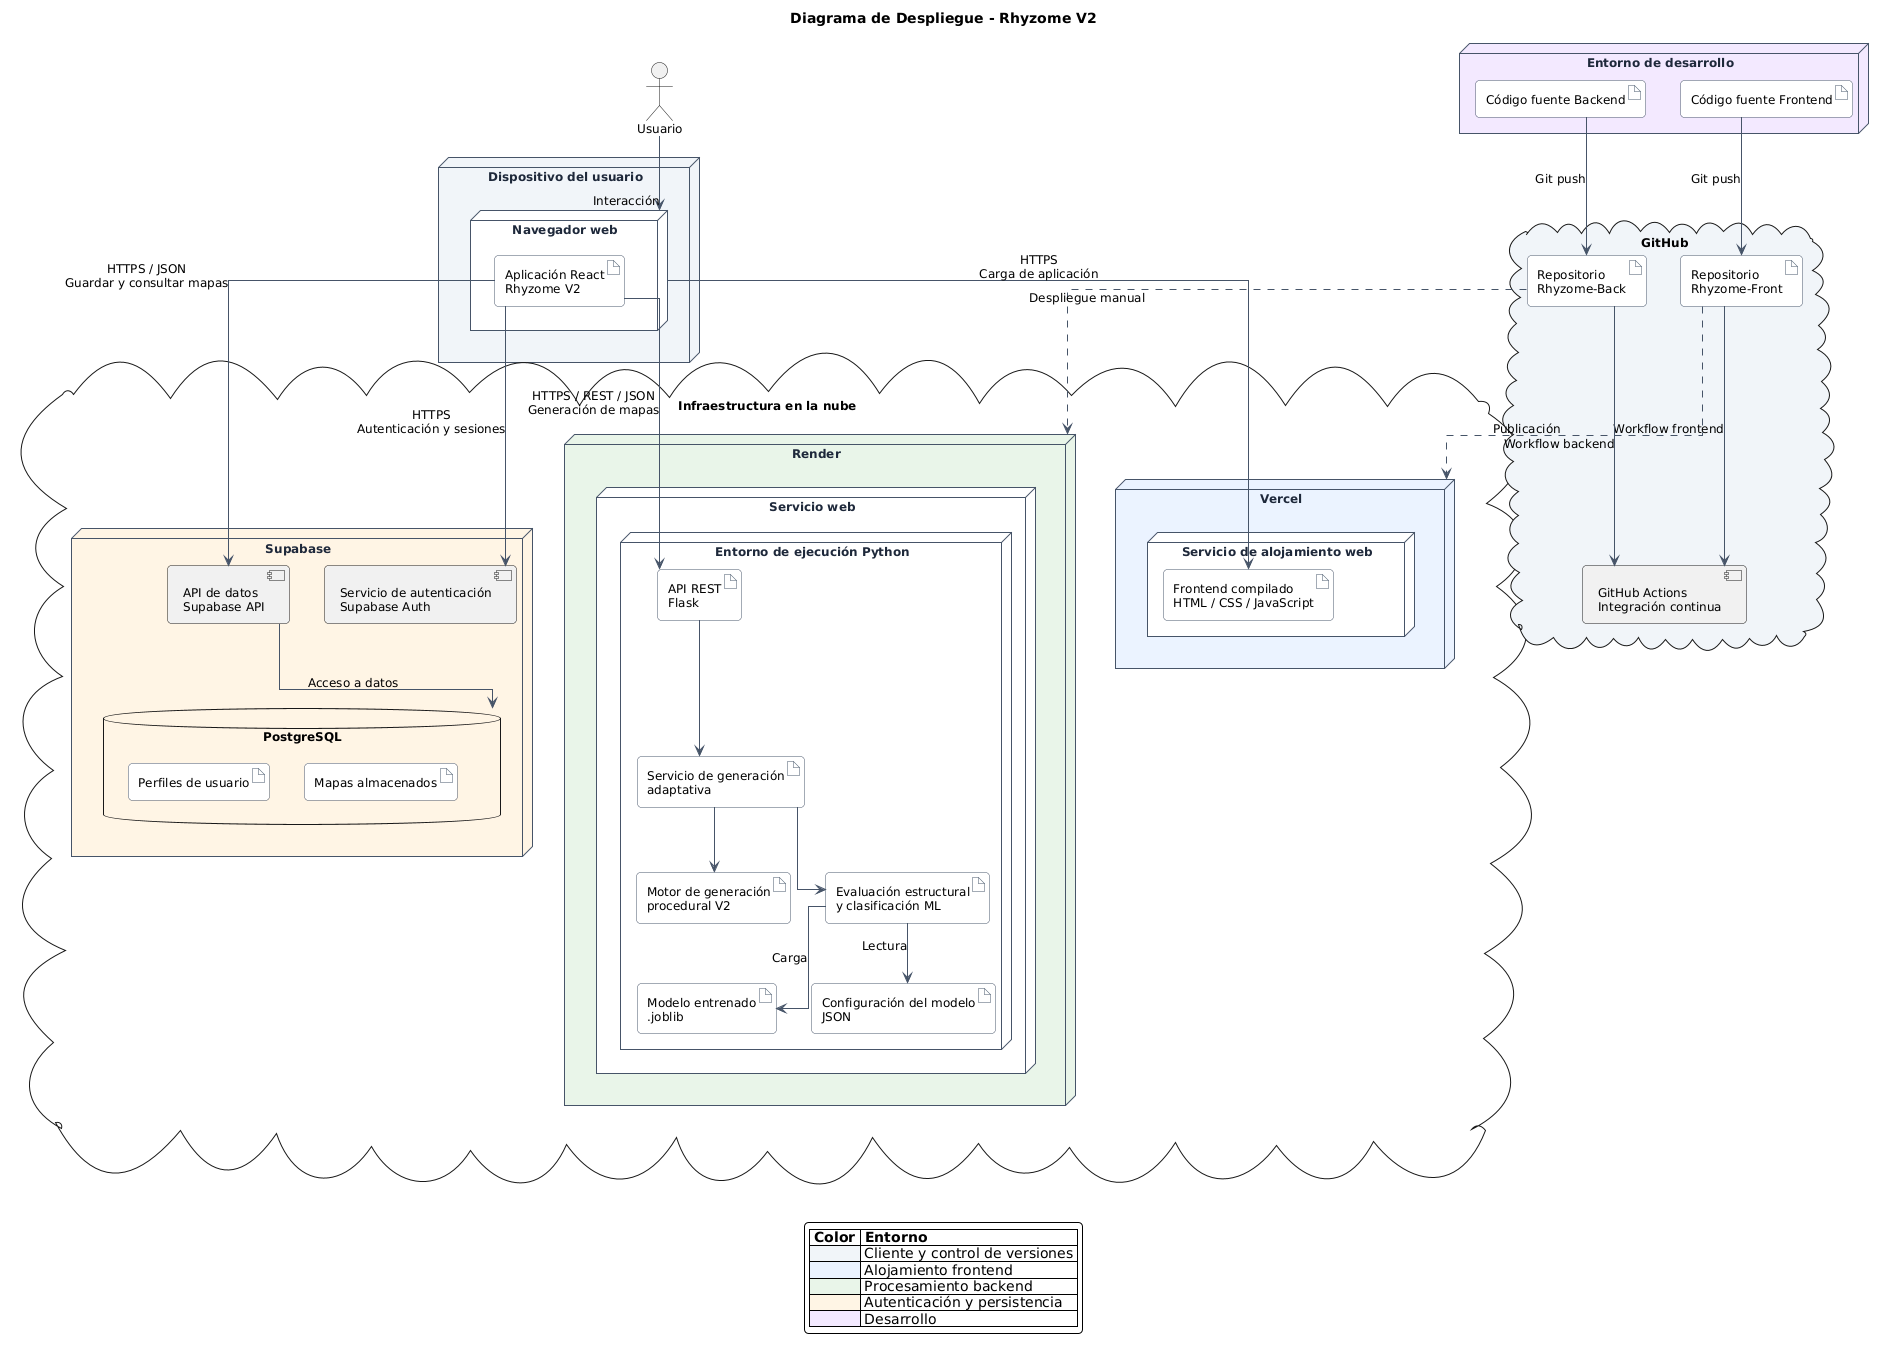
\includegraphics[width=\linewidth,height=0.78\vsize,keepaspectratio]{imagenes/despliegue.png}
		\caption{Diagrama de despliegue de Rhyzome V2}
		\label{fig:despliegue_rhyzome}
	\end{figure}
\end{landscape}

\FloatBarrier

\subsection{Distribución de la infraestructura}

La infraestructura tecnológica de Rhyzome se encuentra distribuida en los siguientes nodos y servicios:

\begin{itemize}
	
	\item \textbf{Dispositivo del usuario:}
	corresponde al equipo desde el cual se accede a la aplicación mediante un navegador web. En este entorno se ejecuta la aplicación desarrollada en React, proporcionando las funcionalidades de autenticación, configuración, generación, visualización y consulta de mapas.
	
	\item \textbf{Vercel:}
	plataforma utilizada para el alojamiento y distribución del frontend. Contiene los archivos compilados de la aplicación web,  permitiendo su acceso mediante el protocolo HTTPS desde diferentes dispositivos.
	
	\item \textbf{Render:}
	plataforma encargada del alojamiento del backend desarrollado en Python y Flask. En este entorno se ejecutan los servicios REST, los algoritmos de generación procedural, la evaluación estructural de los mapas y el componente de aprendizaje automático.
	
	\item \textbf{Supabase:}
	plataforma que proporciona los servicios de autenticación y persistencia de información. Integra una base de datos PostgreSQL utilizada
	para administrar los perfiles de usuario y los mapas almacenados por la aplicación.
	
	\item \textbf{GitHub:}
	plataforma utilizada para el control de versiones del código fuente del frontend y backend. Adicionalmente, mediante GitHub Actions se automatiza la ejecución de pruebas y otros procesos de integración continua.
	
	\item \textbf{Entorno de desarrollo:}
	corresponde al ambiente local en el cual se realizan las actividades de implementación, mantenimiento, pruebas y actualización del
	código fuente antes de su publicación en los ambientes correspondientes.
	
\end{itemize}

\subsection{Comunicación entre los componentes}

La comunicación entre los diferentes nodos del sistema se realiza mediante protocolos web y servicios REST.

Inicialmente, el navegador del usuario establece una conexión HTTPS con Vercel para obtener los archivos necesarios para la ejecución del frontend. Una vez cargada la aplicación, las solicitudes relacionadas con la generación procedural de mapas se envían directamente desde el navegador hacia los servicios REST desplegados en Render, mediante estructuras de datos en formato JSON. El backend procesa los parámetros recibidos, ejecuta los algoritmos de generación procedural, calcula las características estructurales de los mapas y utiliza el modelo de aprendizaje automático para apoyar la evaluación y selección de los escenarios generados. Por otra parte, las operaciones relacionadas con la autenticación, la administración de sesiones y la persistencia de mapas se realizan mediante los servicios proporcionados por Supabase.

Esta distribución permite que las operaciones de generación procedural y aprendizaje automático se ejecuten en el backend, evitando trasladar el procesamiento computacional al dispositivo del usuario.

\subsection{Estrategia de despliegue}

El proyecto utiliza repositorios independientes para la administración del código fuente del frontend y backend, permitiendo gestionar de
manera separada los cambios realizados sobre cada componente.

La integración continua se apoya en GitHub Actions, mediante flujos de trabajo destinados a la ejecución de pruebas automatizadas y
la verificación del código fuente.

La publicación del frontend se realiza mediante Vercel, mientras que el backend se encuentra alojado en Render. Para la versión actual del
prototipo, el despliegue del backend requiere la activación manual del proceso de publicación.

La separación entre los ambientes de desarrollo y producción facilita la validación de los cambios antes de su incorporación a la versión disponible para los usuarios.

\subsection{Consideraciones de infraestructura}

La arquitectura de despliegue seleccionada proporciona una base para la evolución independiente de los componentes del sistema, permitiendo realizar actualizaciones sobre la interfaz, los servicios REST y los modelos de aprendizaje automático. Sin embargo, el rendimiento del sistema depende de los recursos computacionales disponibles en las plataformas de alojamiento, especialmente durante la ejecución de los procesos de generación adaptativa.

En particular, los tiempos de respuesta pueden verse afectados por la inicialización del servicio backend, las dimensiones de los mapas solicitados y la cantidad de candidatos generados durante cada solicitud. Estos factores son relevantes para la evaluación del rendimiento y la identificación de futuras oportunidades de optimización del prototipo.

La evaluación de los tiempos de respuesta y los resultados de las pruebas realizadas se presentan posteriormente en el capítulo de pruebas y validación.

\begin{table}[htbp]
	\centering
	
	\caption{Distribución de los servicios de Rhyzome}
	\label{tab:infraestructura_despliegue}
	
	\renewcommand{\arraystretch}{1.5}
	
	\begin{tabularx}{\textwidth}{
			|>{\raggedright\arraybackslash}p{3cm}|
			>{\raggedright\arraybackslash}p{3cm}|
			>{\raggedright\arraybackslash}X|
		}
		\hline
		
		\rowcolor{gray!15}
		\textbf{Plataforma} &
		\textbf{Componente} &
		\textbf{Responsabilidad} \\
		
		\hline
		
		\textbf{Vercel} &
		Frontend &
		Alojamiento y distribución de la aplicación web desarrollada mediante React, Vite y Tailwind CSS. \\
		
		\hline
		
		\textbf{Render} &
		Backend &
		Ejecución de los servicios REST, algoritmos de generación procedural, evaluación estructural e inferencia de los
		modelos de aprendizaje automático. \\
		
		\hline
		
		\textbf{Supabase} &
		Autenticación &
		Gestión de usuarios, sesiones, inicio de sesión y recuperación de contraseñas. \\
		
		\hline
		
		\textbf{Supabase} &
		PostgreSQL &
		Persistencia y consulta de perfiles de usuario y mapas almacenados en la aplicación. \\
		
		\hline
		
		\textbf{GitHub} &
		Repositorios &
		Control de versiones, administración y trazabilidad de los cambios realizados en el código fuente del frontend y backend. \\
		
		\hline
		
		\textbf{GitHub Actions} &
		Integración continua &
		Ejecución automatizada de pruebas, generación de reportes de cobertura y verificación del código fuente. \\
		
		\hline
		
	\end{tabularx}
	
	\par\smallskip
	\raggedright
	
	\textit{Nota.} La distribución presentada corresponde a la infraestructura tecnológica utilizada en Rhyzome V2. La separación de los servicios permite administrar de manera independiente los componentes de presentación, procesamiento, autenticación y persistencia de información.
	
\end{table}

\FloatBarrier

\section{Tecnologías y frameworks utilizados}
\label{sec:tecnologias_frameworks}

El desarrollo de Rhyzome se fundamenta en la integración de tecnologías orientadas al desarrollo web, la generación procedural de contenido, el aprendizaje automático y la administración de servicios en la nube.

La selección de estas tecnologías se realizó considerando criterios de compatibilidad, modularidad, facilidad de integración, mantenimiento y disponibilidad de herramientas para el desarrollo del prototipo.

La arquitectura tecnológica permite separar las responsabilidades de presentación, procesamiento, persistencia de información e inferencia de los modelos de aprendizaje automático.

\subsection{Stack tecnológico}

La Tabla~\ref{tab:stack_tecnologico} presenta las principales tecnologías y frameworks utilizados en la implementación de Rhyzome, identificando su categoría y responsabilidad dentro del sistema.

\begin{table}[htbp]
	\centering
	
	\caption{Tecnologías y frameworks utilizados en Rhyzome}
	\label{tab:stack_tecnologico}
	
	\renewcommand{\arraystretch}{1.5}
	
	\begin{tabularx}{\textwidth}{
			|>{\raggedright\arraybackslash}p{2.8cm}|
			>{\raggedright\arraybackslash}p{2.8cm}|
			>{\raggedright\arraybackslash}X|
		}
		\hline
		
		\rowcolor{gray!15}
		\textbf{Tecnología} &
		\textbf{Categoría} &
		\textbf{Responsabilidad} \\
		
		\hline
		
		\textbf{Python} &
		Lenguaje de programación &
		Implementación del backend, los algoritmos de generación procedural y el componente de aprendizaje automático. \\
		
		\hline
		
		\textbf{JavaScript} &
		Lenguaje de programación &
		Implementación de la lógica de interacción y comportamiento de la aplicación web. \\
		
		\hline
		
		\textbf{Flask} &
		Framework backend &
		Implementación de los servicios REST y coordinación de las solicitudes de generación de mapas. \\
		
		\hline
		
		\textbf{React} &
		Biblioteca frontend &
		Construcción de interfaces mediante componentes reutilizables y gestión del estado de la aplicación. \\
		
		\hline
		
		\textbf{Vite} &
		Herramienta de construcción &
		Configuración del entorno de desarrollo y compilación de la aplicación frontend. \\
		
		\hline
		
		\textbf{Tailwind CSS} &
		Framework CSS &
		Definición de estilos, distribución visual y diseño adaptable de la interfaz de usuario. \\
		
		\hline
		
		\textbf{React Router} &
		Enrutamiento &
		Administración de la navegación y protección de rutas privadas en la aplicación. \\
		
		\hline
		
		\textbf{NumPy} &
		Computación científica &
		Procesamiento de matrices, operaciones numéricas y representación de estructuras de mapas. \\
		
		\hline
		
		\textbf{SciPy} &
		Computación científica &
		Apoyo al procesamiento numérico y análisis de características estructurales. \\
		
		\hline
		
		\textbf{Scikit-learn} &
		Aprendizaje automático &
		Implementación y utilización de modelos supervisados para la clasificación de complejidad de los mapas. \\
		
		\hline
		
		\textbf{Joblib} &
		Serialización &
		Almacenamiento y carga de los artefactos de los modelos de aprendizaje automático. \\
		
		\hline
		
		\textbf{Supabase} &
		Backend como servicio &
		Administración de la autenticación, sesiones y persistencia de información. \\
		
		\hline
		
		\textbf{PostgreSQL} &
		Base de datos relacional &
		Almacenamiento de perfiles de usuario y mapas registrados en la aplicación. \\
		
		\hline
		
	\end{tabularx}
	
	\par\smallskip
	\raggedright
	
	\textit{Nota.} Las tecnologías presentadas corresponden al stack tecnológico de Rhyzome y se encuentran agrupadas de acuerdo con su responsabilidad dentro de la arquitectura del sistema.
	
\end{table}

\FloatBarrier

\subsection{Herramientas de desarrollo y soporte}

Además de las tecnologías utilizadas en la implementación del sistema, el proyecto incorpora herramientas de soporte orientadas al control de versiones, la automatización de pruebas, el despliegue y la gestión del desarrollo.

La Tabla~\ref{tab:herramientas_soporte} presenta las herramientas que respaldan estas actividades.

\begin{table}[htbp]
	\centering
	
	\caption{Herramientas de desarrollo y soporte de Rhyzome}
	\label{tab:herramientas_soporte}
	
	\renewcommand{\arraystretch}{1.5}
	
	\begin{tabularx}{\textwidth}{
			|>{\raggedright\arraybackslash}p{2.8cm}|
			>{\raggedright\arraybackslash}p{2.8cm}|
			>{\raggedright\arraybackslash}X|
		}
		\hline
		
		\rowcolor{gray!15}
		\textbf{Herramienta} &
		\textbf{Categoría} &
		\textbf{Responsabilidad} \\
		
		\hline
		
		\textbf{Git} &
		Control de versiones &
		Administración del historial de cambios del código fuente. \\
		
		\hline
		
		\textbf{GitHub} &
		Repositorios &
		Almacenamiento y administración de los repositorios del frontend y backend. \\
		
		\hline
		
		\textbf{GitHub Actions} &
		Integración continua &
		Automatización de pruebas y generación de reportes de ejecución y cobertura. \\
		
		\hline
		
		\textbf{Pytest} &
		Pruebas backend &
		Ejecución de pruebas unitarias, funcionales y de integración sobre los componentes desarrollados en Python. \\
		
		\hline
		
		\textbf{Vitest} &
		Pruebas frontend &
		Validación automatizada de componentes y servicios de la aplicación web. \\
		
		\hline
		
		\textbf{Postman} &
		Validación de API &
		Ejecución manual de solicitudes HTTP y verificación de los contratos de comunicación REST. \\
		
		\hline
		
		\textbf{Vercel} &
		Despliegue &
		Alojamiento y distribución del frontend. \\
		
		\hline
		
		\textbf{Render} &
		Despliegue &
		Alojamiento y ejecución de los servicios backend. \\
		
		\hline
		
		\textbf{Jira} &
		Gestión ágil &
		Administración del Product Backlog, historias de usuario, sprints y seguimiento del proyecto. \\
		
		\hline
		
		\textbf{Confluence} &
		Documentación &
		Organización de la documentación técnica y evidencias del proyecto. \\
		
		\hline
		
	\end{tabularx}
	
	\par\smallskip
	\raggedright
	
	\textit{Nota.} Las herramientas de soporte contribuyen a la trazabilidad, verificación, documentación y mantenimiento del proyecto durante su ciclo de desarrollo.
	
\end{table}

\FloatBarrier

\subsection{Justificación de la selección tecnológica}

La selección de las tecnologías utilizadas en Rhyzome responde a las necesidades funcionales y técnicas identificadas durante el diseño de la solución.

\subsubsection{Tecnologías de frontend}

React fue seleccionado por su enfoque basado en componentes reutilizables, el cual facilita la construcción de interfaces modulares y la separación de responsabilidades visuales.

Su integración con Vite y Tailwind CSS permite disponer de un entorno de desarrollo orientado a la construcción de interfaces web interactivas y al mantenimiento de una estructura visual consistente.

\subsubsection{Tecnologías de backend}

Python fue seleccionado debido a su ecosistema de bibliotecas orientadas al procesamiento numérico, la generación procedural y el aprendizaje automático.

Flask proporciona una estructura flexible para la implementación de servicios REST, permitiendo organizar las funcionalidades del backend mediante módulos y mantener separada la lógica de procesamiento de la interfaz de usuario.

\subsubsection{Generación procedural y aprendizaje automático}

NumPy y SciPy proporcionan herramientas para el procesamiento de matrices y el análisis numérico de las estructuras generadas por los algoritmos procedurales.

Scikit-learn permite integrar modelos de clasificación supervisada dentro del proceso de generación adaptativa, mientras que Joblib facilita la serialización y carga de los modelos entrenados.

La utilización de estas tecnologías permite integrar la generación procedural y la inferencia de aprendizaje automático dentro de un mismo entorno de ejecución.

\subsubsection{Autenticación y persistencia}

Supabase fue seleccionado como servicio externo para la administración de usuarios, sesiones y persistencia de información.

La integración con PostgreSQL permite gestionar los datos asociados a los usuarios y los mapas almacenados, reduciendo la necesidad de implementar desde cero un servicio independiente de administración de datos.

\subsubsection{Despliegue y aseguramiento de la calidad}

La utilización de Vercel y Render permite mantener separados los ambientes de alojamiento del frontend y backend.

GitHub Actions, Pytest y Vitest complementan esta arquitectura mediante mecanismos de integración continua y validación automatizada, contribuyendo a la detección de errores y al mantenimiento del código fuente.

En conjunto, las tecnologías seleccionadas proporcionan una base modular para el desarrollo del prototipo, facilitando la integración de sus componentes y permitiendo su evolución de acuerdo con las necesidades identificadas durante el proyecto.

\section{Diseño de la interfaz de usuario}
\label{sec:diseno_interfaz_usuario}

El diseño de la interfaz de usuario de Rhyzome se orienta a proporcionar un entorno interactivo que facilite la configuración, generación, visualización, evaluación y administración de mapas procedurales para videojuegos 2D.

La interfaz permite que los usuarios interactúen con los algoritmos de generación procedural y el componente de aprendizaje automático sin necesidad de conocer los detalles internos de su implementación.

Su desarrollo se realizó mediante React, Vite y Tailwind CSS, utilizando una estructura basada en componentes reutilizables que permite separar las responsabilidades visuales y funcionales de la aplicación.

\subsection{Metodología de diseño}

El diseño de la interfaz se desarrolló mediante un proceso incremental e iterativo, articulado con la metodología ágil adoptada en el proyecto. Inicialmente, se identificaron las necesidades funcionales de los usuarios relacionadas con la configuración de parámetros, la generación procedural, la visualización y la administración de mapas. A partir de estas necesidades, se definió la organización de la información y la distribución de las funcionalidades principales dentro de la aplicación.

El proceso de diseño contempló las siguientes actividades:

\begin{enumerate}
	
	\item Identificación de las necesidades y funcionalidades requeridas por los usuarios.
	
	\item Definición de la arquitectura de información y los mecanismos de navegación.
	
	\item Construcción de una interfaz inicial para la configuración y visualización de mapas.
	
	\item Integración de los servicios de generación procedural y aprendizaje automático.
	
	\item Mejoramiento progresivo de los componentes visuales y mecanismos de interacción.
	
	\item Incorporación de funcionalidades de autenticación, almacenamiento, consulta y exportación de mapas.
	
	\item Validación funcional de las interfaces implementadas.
	
\end{enumerate}

La evolución de la interfaz permitió incorporar nuevas funcionalidades de manera progresiva, manteniendo la coherencia con los requerimientos del proyecto y las historias de usuario definidas durante las iteraciones de desarrollo.

\subsection{Arquitectura de información y navegación}

La arquitectura de información de Rhyzome organiza las funcionalidades del sistema mediante una separación entre interfaces públicas, interfaces privadas y operaciones asociadas a la generación procedural de mapas.

Las interfaces públicas permiten realizar operaciones de autenticación, registro y recuperación de contraseña, mientras que las interfaces privadas proporcionan acceso a las funcionalidades principales del generador.

La Figura~\ref{fig:navegacion_interfaz} representa la organización funcional de las interfaces y las relaciones de navegación existentes entre ellas.

\begin{figure}[H]
	\centering
	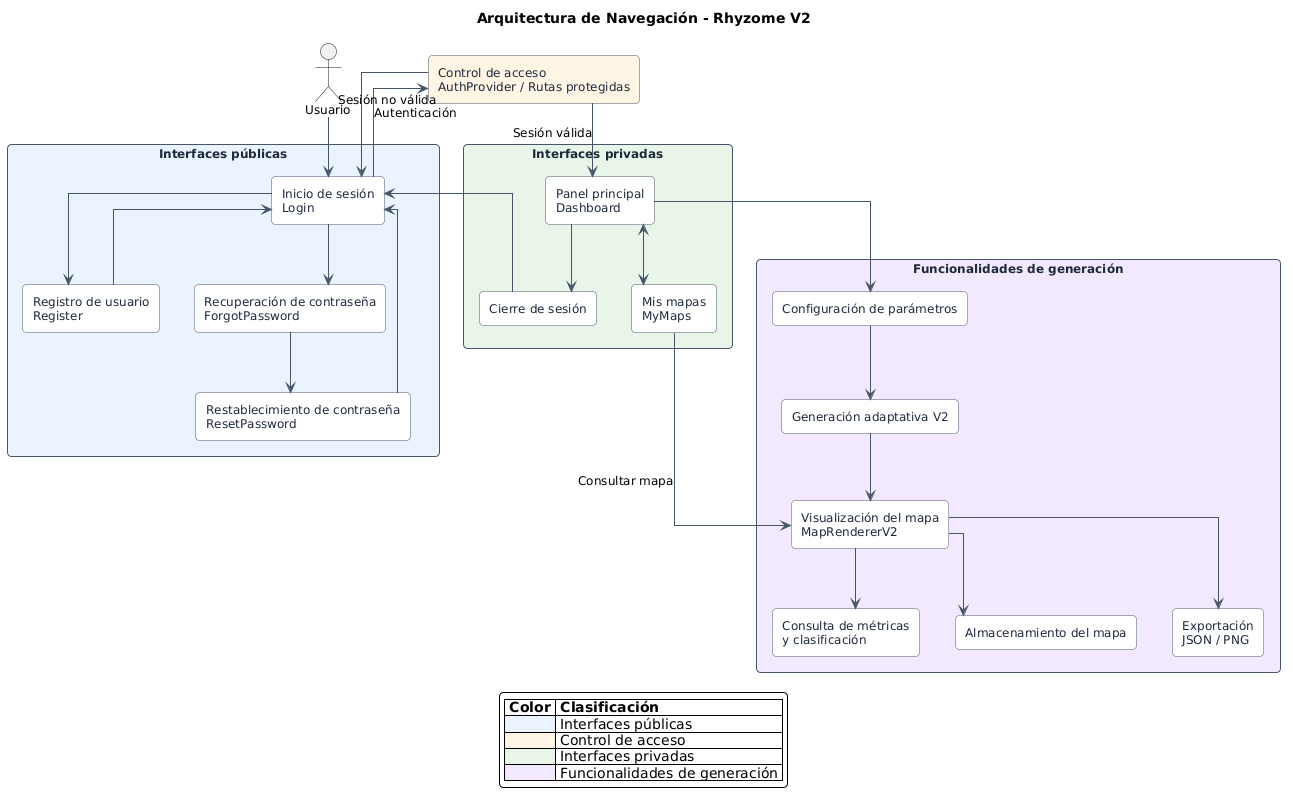
\includegraphics[width=\textwidth]{imagenes/navegacion.png}
	\caption{Arquitectura de navegación de Rhyzome V2}
	\label{fig:navegacion_interfaz}
\end{figure}

\FloatBarrier

Como se observa en la figura, el acceso a las funcionalidades principales se encuentra condicionado por la existencia de una sesión válida.

Una vez autenticado, el usuario puede acceder al panel principal de generación y consultar los mapas almacenados.

Esta organización permite diferenciar las operaciones relacionadas con la administración de usuarios de aquellas orientadas a la generación, visualización y gestión de mapas procedurales.

\subsection{Criterios y decisiones de diseño}

El diseño de la interfaz de Rhyzome consideró criterios orientados a facilitar la interacción, mantener la consistencia visual y organizar las funcionalidades de acuerdo con las tareas realizadas por el usuario.

La Tabla~\ref{tab:criterios_diseno_interfaz} presenta los principales criterios considerados durante el desarrollo de la interfaz.

\begin{table}[htbp]
	\centering
	
	\caption{Criterios de diseño de la interfaz de Rhyzome}
	\label{tab:criterios_diseno_interfaz}
	
	\renewcommand{\arraystretch}{1.5}
	
	\begin{tabularx}{\textwidth}{
			|>{\raggedright\arraybackslash}p{3.5cm}|
			>{\raggedright\arraybackslash}X|
		}
		\hline
		
		\rowcolor{gray!15}
		\textbf{Criterio} &
		\textbf{Aplicación en Rhyzome} \\
		
		\hline
		
		\textbf{Consistencia visual} &
		Utilización de estilos, colores y componentes reutilizables para mantener una presentación uniforme entre las interfaces. \\
		
		\hline
		
		\textbf{Jerarquía visual} &
		Organización de los controles y resultados de acuerdo con su importancia dentro del proceso de generación procedural. \\
		
		\hline
		
		\textbf{Facilidad de interacción} &
		Agrupación de los parámetros y acciones principales dentro del panel de generación. \\
		
		\hline
		
		\textbf{Retroalimentación} &
		Presentación de información relacionada con el procesamiento de solicitudes, resultados y errores de la aplicación. \\
		
		\hline
		
		\textbf{Diferenciación de terrenos} &
		Representación visual de los escenarios mediante colores y elementos asociados a las características del terreno generado. \\
		
		\hline
		
		\textbf{Control de acceso} &
		Separación de las interfaces públicas y privadas, condicionando el acceso a una sesión válida. \\
		
		\hline
		
		\textbf{Modularidad} &
		Implementación de componentes React reutilizables para facilitar el mantenimiento y evolución de la interfaz. \\
		
		\hline
		
		\textbf{Control del usuario} &
		Disponibilidad de opciones para configurar, generar, consultar, almacenar y exportar mapas. \\
		
		\hline
		
	\end{tabularx}
	
	\par\smallskip
	\raggedright
	
	\textit{Nota.} Los criterios descritos corresponden a decisiones de diseño aplicadas durante el desarrollo incremental de la interfaz de Rhyzome.
	
\end{table}

\FloatBarrier

La aplicación de estos criterios busca reducir la complejidad de interacción con los algoritmos de generación procedural y el componente inteligente.

Asimismo, la separación de las funcionalidades permite organizar la experiencia de usuario alrededor de las principales tareas del sistema, evitando que los detalles técnicos de implementación interfieran directamente con el proceso de generación de mapas.

\subsection{Interfaz definitiva del prototipo}
\label{subsec:resultados_diseno_interfaz}

La interfaz de usuario de Rhyzome integra las funcionalidades de configuración, generación procedural, visualización, evaluación, almacenamiento y exportación de mapas dentro de un entorno web unificado.

El diseño presenta una organización funcional orientada a facilitar la interacción con los algoritmos de generación
procedural y el componente de aprendizaje automático, permitiendo configurar las características de los escenarios
sin requerir conocimientos sobre su implementación interna.

La representación gráfica de los mapas utiliza elementos visuales asociados a los diferentes tipos de terreno, permitiendo identificar las características y estructuras que conforman cada escenario generado.

La Figura~\ref{fig:resultado_final_interfaz} presenta la interfaz correspondiente a la versión definitiva del prototipo Rhyzome.

\begin{figure}[H]
	\centering
	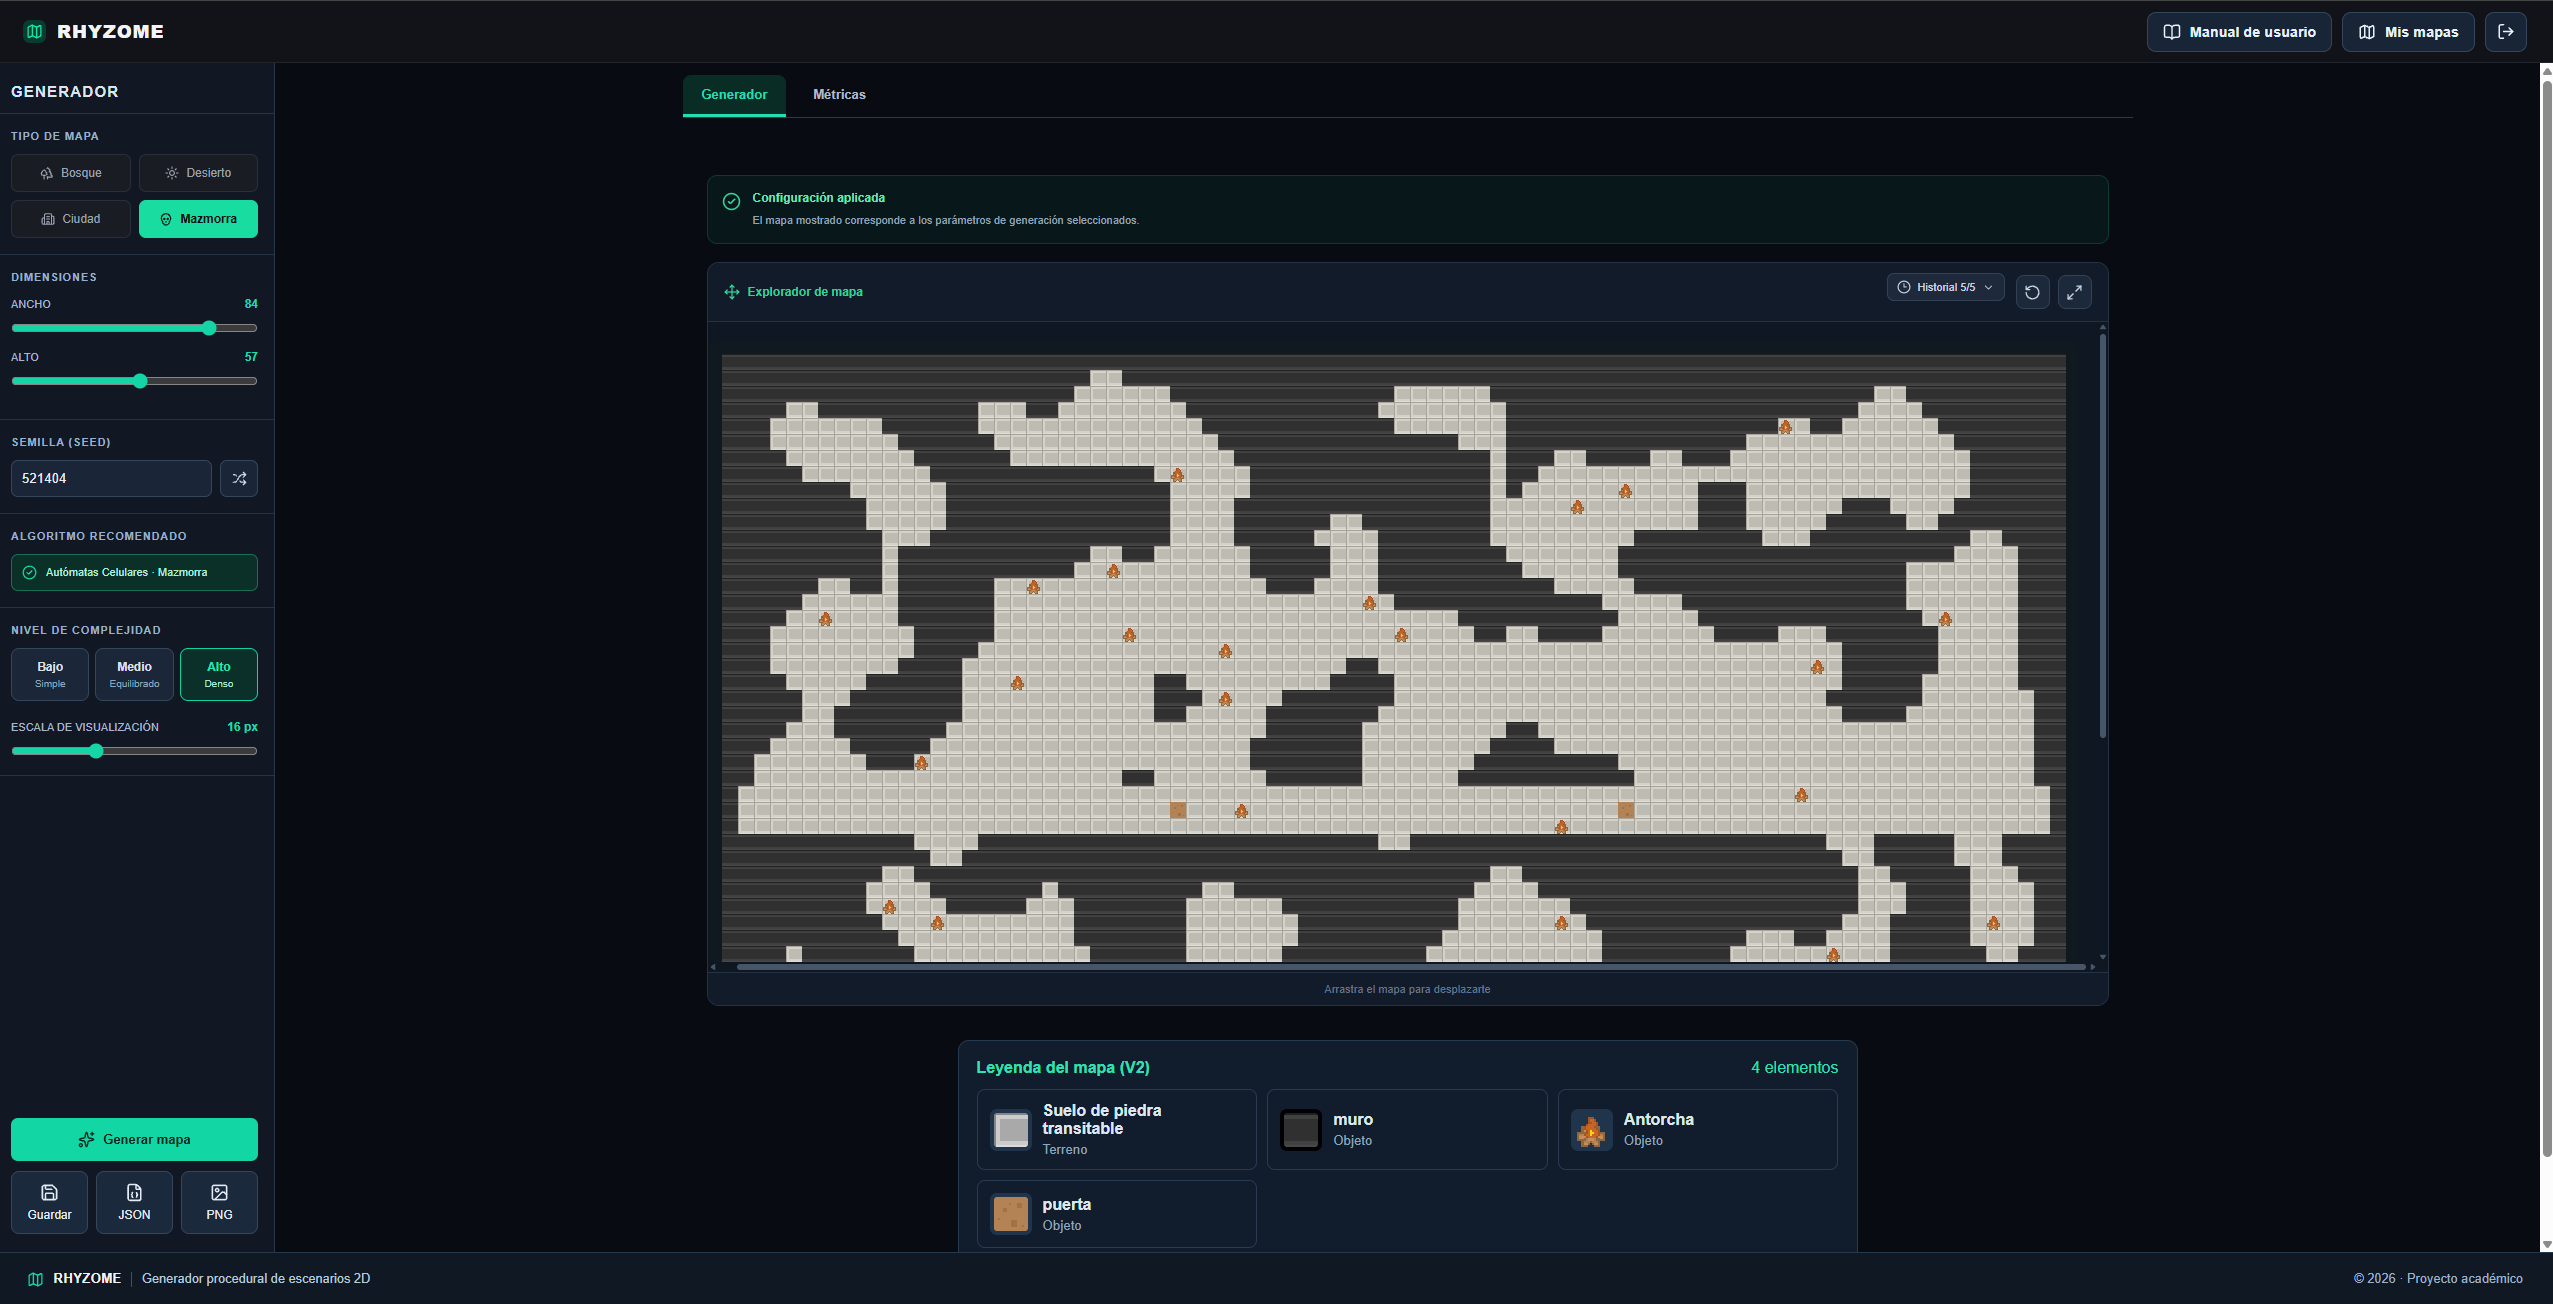
\includegraphics[width=\textwidth]{imagenes/mazmorra.png}
	\caption{Interfaz definitiva del prototipo Rhyzome}
	\label{fig:resultado_final_interfaz}
\end{figure}

El dashboard reúne los controles de terreno, dimensiones, complejidad y semilla, el área de visualización del mapa y las opciones de consulta de métricas, almacenamiento y exportación JSON y PNG. Los criterios de diseño se recogen en la Tabla~\ref{tab:criterios_diseno_interfaz}; la comprobación funcional corresponde al Capítulo~\ref{cap:06_pruebas_validacion}.

\FloatBarrier

\section{Estrategia de integración del modelo de IA}
\label{sec:integracion_ia}

\subsection{Flujo de generación adaptativa}
\label{subsec:estrategia_generacion_adaptativa}

La generación adaptativa integra la construcción procedural de mapas con la clasificación de complejidad mediante aprendizaje automático. El servicio de generación coordina la evaluación de los candidatos y selecciona el escenario que mejor se ajusta a la solicitud del usuario.

La Figura~\ref{fig:integracion_modelo_ia} presenta el diagrama de secuencia de este proceso. A diferencia del flujo funcional de la Figura~\ref{fig:flujo_funcional}, esta representación describe los intercambios entre los componentes de software durante una solicitud de generación.

\FloatBarrier

\begin{landscape}
	\begin{figure}[H]
		\centering
		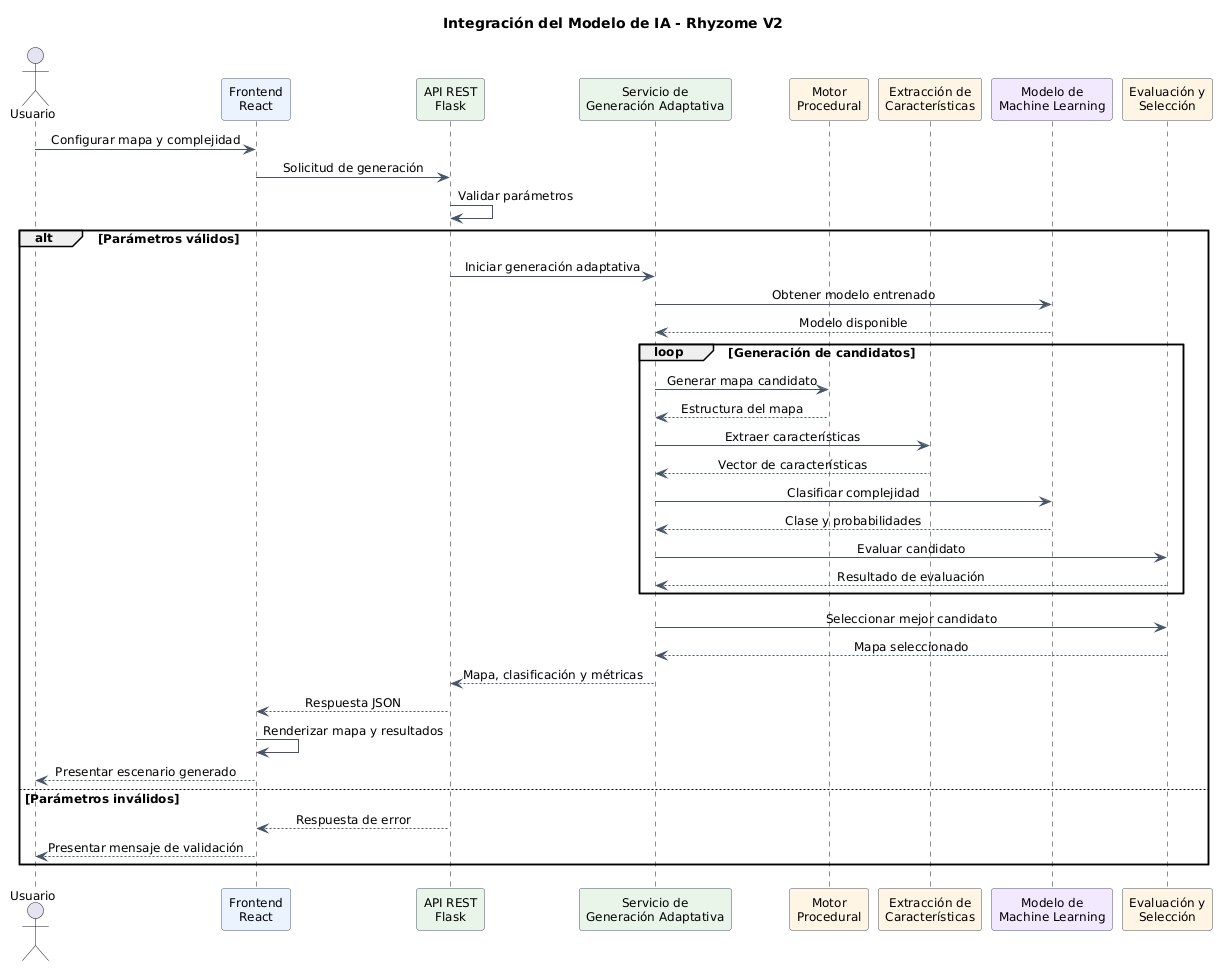
\includegraphics[
		width=\linewidth,
		height=0.78\vsize,
		keepaspectratio
		]{imagenes/integracion_modelo_ia.png}
		\caption{Diagrama de secuencia de integración del modelo de IA en Rhyzome}
		\label{fig:integracion_modelo_ia}
	\end{figure}
\end{landscape}

\FloatBarrier

La API REST recibe y valida los parámetros de generación. El servicio adaptativo coordina la construcción de los mapas candidatos mediante el algoritmo procedural correspondiente al terreno seleccionado. Para cada candidato se extraen sus características, se estima su complejidad mediante el clasificador correspondiente y se realiza la evaluación estructural. La selección considera los resultados obtenidos dentro del límite de intentos configurado. La respuesta se entrega en formato JSON e incluye el mapa seleccionado, su clasificación y sus métricas estructurales.

\subsubsection{Formalización del mecanismo de selección}
\label{subsubsec:formalizacion_seleccion}

El mecanismo de selección es el componente de la generación adaptativa encargado de comparar los mapas candidatos producidos por los algoritmos procedurales, con el propósito de identificar el escenario que mejor se ajusta al nivel de complejidad solicitado por el usuario. Para ello, integra los resultados de la clasificación mediante aprendizaje automático y la evaluación de las características estructurales de cada mapa. La siguiente formalización matemática describe los elementos que intervienen en este proceso, la estimación de la probabilidad de pertenencia a la clase objetivo y la representación conceptual del criterio utilizado para seleccionar el mapa resultante.

Sea $\mathcal{M}$ el conjunto de mapas candidatos obtenidos durante una solicitud de generación:

\begin{equation}
	\mathcal{M} = \{M_1,M_2,\ldots,M_n\}
	\label{eq:conjunto_candidatos}
\end{equation}

En esta expresión, $n$ representa la cantidad de candidatos considerados durante el proceso de generación adaptativa. Para cada mapa candidato se obtiene su representación numérica, su clasificación de complejidad y los resultados de evaluación estructural. A partir de su vector de características, el modelo de aprendizaje automático proporciona una estimación de la probabilidad de pertenencia a la clase de complejidad solicitada por el usuario, expresada mediante:

\begin{equation}
	p_i = P_{\theta}(y=c^{*}\mid\mathbf{x}_i)
	\label{eq:probabilidad_clase_objetivo}
\end{equation}

Los términos de la expresión se definen de la siguiente manera:

\begin{itemize}
	
	\item $c^{*}$ representa la clase de complejidad solicitada por el usuario.
	
	\item $\mathbf{x}_i$ corresponde al vector de características del mapa candidato $M_i$.
	
	\item $p_i$ representa la probabilidad estimada de pertenencia a la clase objetivo.
	
	\item $\theta$ representa los parámetros del modelo de aprendizaje automático entrenado.
	
	\item $y$ representa la variable asociada a la clase de complejidad.
	
\end{itemize}

La estrategia de selección utiliza la coincidencia entre la clase predicha y la clase objetivo, las probabilidades proporcionadas por el modelo y los resultados de evaluación estructural. Estos elementos permiten establecer criterios de preferencia entre los diferentes escenarios candidatos. Como representación conceptual, la selección del mapa resultante puede expresarse mediante:

\begin{equation}
	M^{*} =
	\underset{M_i \in \mathcal{M}}{\operatorname{arg\,max}}
	\; S(M_i,c^{*})
	\label{eq:seleccion_mapa}
\end{equation}

En esta expresión, $S$ representa el criterio de selección utilizado para comparar los escenarios candidatos y $M^{*}$ corresponde al mapa seleccionado. Esta expresión constituye una abstracción del mecanismo de selección y no implica necesariamente la utilización de una suma ponderada de métricas.

Cuando los candidatos no coinciden exactamente con la complejidad solicitada, el mecanismo de selección identifica el escenario disponible que presenta las condiciones más favorables de acuerdo con los criterios establecidos. Por consiguiente, la generación adaptativa se orienta a mejorar la correspondencia entre las características solicitadas y el escenario obtenido, sin garantizar una coincidencia absoluta en todas las solicitudes.

\subsection{Gestión de los modelos en producción}
\label{subsec:gestion_modelos_produccion}
El entrenamiento de los modelos de aprendizaje automático se realiza fuera del entorno de producción, separando la experimentación de la inferencia ejecutada por la aplicación. El backend carga artefactos serializados mediante Joblib y ejecuta la inferencia con scikit-learn \parencite{pedregosa2011}. La Tabla~\ref{tab:gestion_modelos_ia} identifica los artefactos, módulos y servicios documentados para la integración del componente inteligente.

\begin{table}[htbp]
	\centering
	
	\caption{Elementos técnicos de integración del modelo de IA}
	\label{tab:gestion_modelos_ia}
	
	\renewcommand{\arraystretch}{1.5}
	
	\begin{tabularx}{\textwidth}{
			|>{\raggedright\arraybackslash}p{5.5cm}|
			>{\raggedright\arraybackslash}X|
		}
		\hline
		
		\rowcolor{gray!15}
		\textbf{Elemento} &
		\textbf{Responsabilidad o justificación} \\
		\hline
		
		\texttt{best\_\allowbreak cellular.joblib} &
		Clasificador de complejidad para mapas generados mediante Autómatas Celulares. \\
		\hline
		
		\texttt{best\_\allowbreak perlin.joblib} &
		Clasificador de complejidad para mapas generados mediante Perlin Noise. \\
		\hline
		
		\texttt{feature\_\allowbreak config.json} &
		Configuración del orden de las características de entrada y la codificación de las clases. \\
		\hline
		
		\texttt{experiment\_\allowbreak manifest.json} &
		Registro de la selección de los modelos obtenidos durante el proceso experimental. \\
		\hline
		
		\texttt{adaptive\_\allowbreak generator\_\allowbreak ml.py} &
		Coordinación de la generación de candidatos, inferencia y selección adaptativa de mapas. \\
		\hline
		
		\texttt{evaluation\_\allowbreak metrics.py} &
		Cálculo de las métricas utilizadas para la evaluación estructural de los mapas. \\
		\hline
		
		\texttt{/api/maps/\allowbreak generate-adaptive} &
		Endpoint REST responsable de atender las solicitudes de generación adaptativa. \\
		\hline
		
	\end{tabularx}
	
	\par\smallskip
	\raggedright
	
	\textit{Nota.} La tabla presenta los artefactos, módulos de software y servicios REST asociados con la integración del componente de aprendizaje automático en Rhyzome.
	
\end{table}

\FloatBarrier

\subsection{Decisiones técnicas de integración}
\label{subsec:decisiones_integracion_ia}

La actualización de modelos requiere conservar el orden de las características, la codificación de clases y la compatibilidad de las dependencias con el entorno de entrenamiento. No se realiza entrenamiento continuo durante las solicitudes. La selección experimental se documenta en el Capítulo~\ref{cap:04_modelo_ia} y la validación funcional en el Capítulo~\ref{cap:06_pruebas_validacion}.

\FloatBarrier

\section{Seguridad, escalabilidad y mantenimiento}
\label{sec:seguridad_escalabilidad_mantenimiento}

\subsection{Seguridad de la aplicación}
La autenticación se apoya en Supabase Auth y la navegación privada requiere una sesión válida. La protección de rutas del frontend no sustituye la autorización del backend ni las políticas de acceso a datos. La comunicación en producción utiliza HTTPS. Las credenciales privadas deben mantenerse fuera del repositorio y del código distribuido al navegador. La validación de parámetros del servicio limita las solicitudes inválidas. La verificación de los mecanismos de autorización y las políticas de acceso corresponde al Capítulo~\ref{cap:06_pruebas_validacion}.

\subsection{Escalabilidad y rendimiento}
La separación del frontend en Vercel y del procesamiento en Render permite administrar ambos servicios de forma independiente. El costo de generación depende de las dimensiones, la cantidad de candidatos y la extracción de características. La reutilización de modelos cargados evita repetir su deserialización. La inicialización del servicio en Render puede afectar la latencia. No se afirma una capacidad de escalamiento determinada sin pruebas de carga; los resultados de rendimiento se abordan en el Capítulo~\ref{cap:06_pruebas_validacion}.

\subsection{Mantenimiento y evolución}
Los repositorios de frontend y backend se gestionan mediante GitHub. GitHub Actions ejecuta pruebas automatizadas y genera reportes; la publicación del backend requiere activación manual. El mantenimiento contempla el control de versiones de dependencias, artefactos de aprendizaje automático y contratos REST. Los cambios en características o algoritmos requieren evaluar su compatibilidad con los modelos entrenados y ejecutar pruebas de regresión antes del despliegue.
